
\sekcicka{První příloha -- Detailnější výsledky měření}

Tato příloha obsahuje tři doplňující grafy. Pro každého pozorovatele zvlášť je
zde uveden jeho počet fixací v jednotlivých úkolech, a obtížnost, kterou daný
úkol měl. Protože je ale bodový graf v případě počtu
fixací kvůli vysokému rozptylu velmi nepřehledný, je místo toho v tomto grafu
pro každý test a každého účastníka pouze přímka, která je výsledkem lineární regrese. Stejně jako grafy v samotné práci, ani tyto nezahrnují prvních pět úkolů. 

Dále je zde graf závislosti průměrného počtu fixací na obtížnosti.

\def\graphfigure#1#2#3{
\begin{figure}[h!]
\centering
 \makebox[\textwidth][c]{\includegraphics{graphs/#1}}
\caption{#2}
\label{#3}
\end{figure}
}

\graphfigure{Kontrast_fix}{Závislost počtu fixací, než bylo oznámeno nalezení
cíle, na obtížnosti. Krajní hodnoty, které se jako jediné výrazně odlišují od
ostatních, jsou výsledkem velmi mála měření (krajní hodnoty pouze
jednotek, hodnoty vedle nich řádově dvaceti. Mezi hodnotami kontrastu 0.57 a
0.71 je naopak ke každé hodnotě k dispozici alespoň 50 měření). }{kontr}

\begin{center}
\begin{figure}
\centering
 \makebox[\textwidth][c]{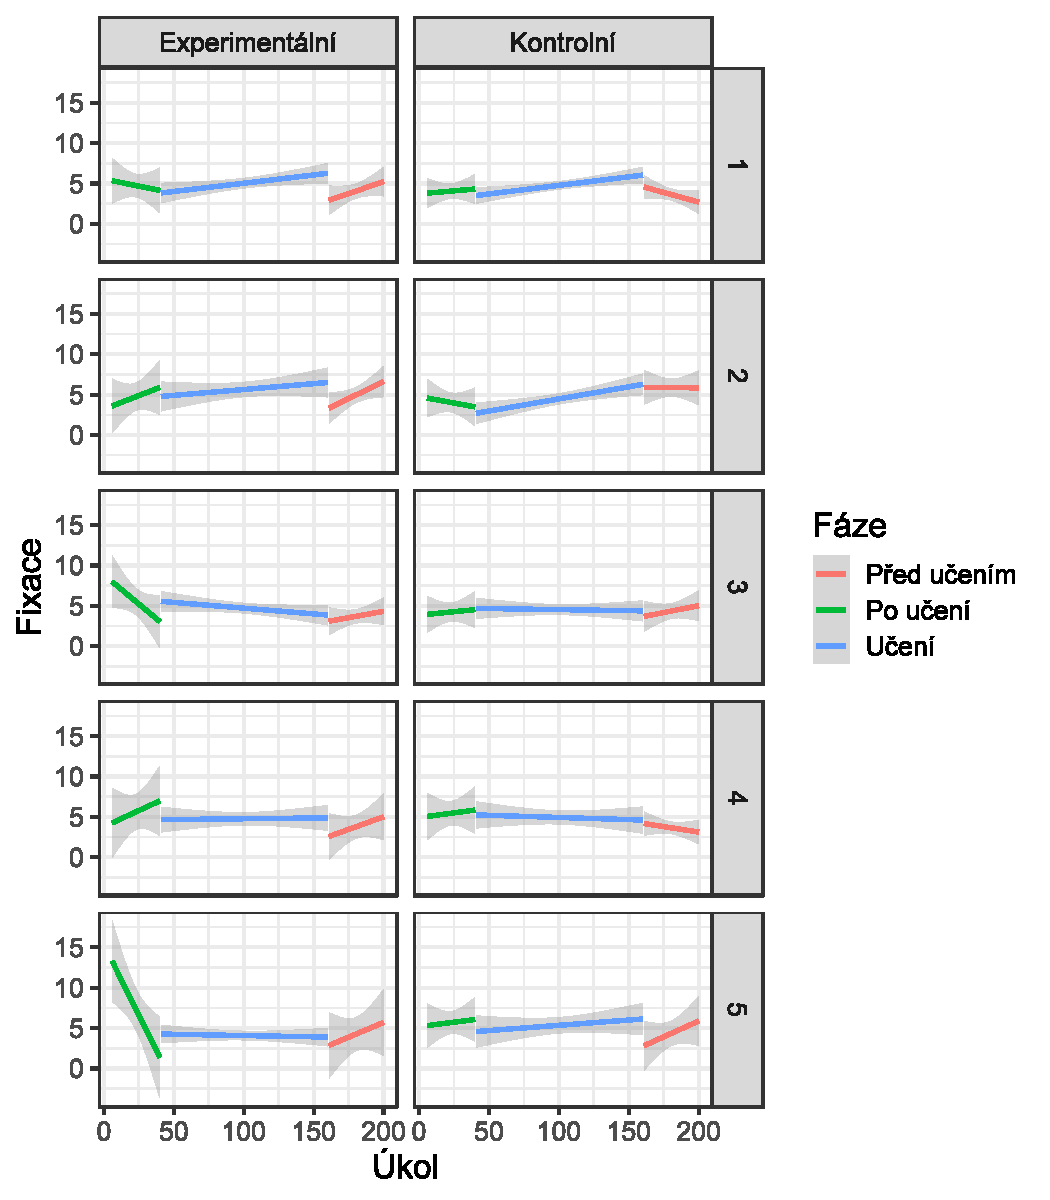
\includegraphics{graphs/Fixations_grid}}
\caption{Závislost počtu fixací, než bylo oznámeno nalezení cíle, na celkovém čísle úkolu.}
\end{figure} 

\begin{figure}
\centering
 \makebox[\textwidth][c]{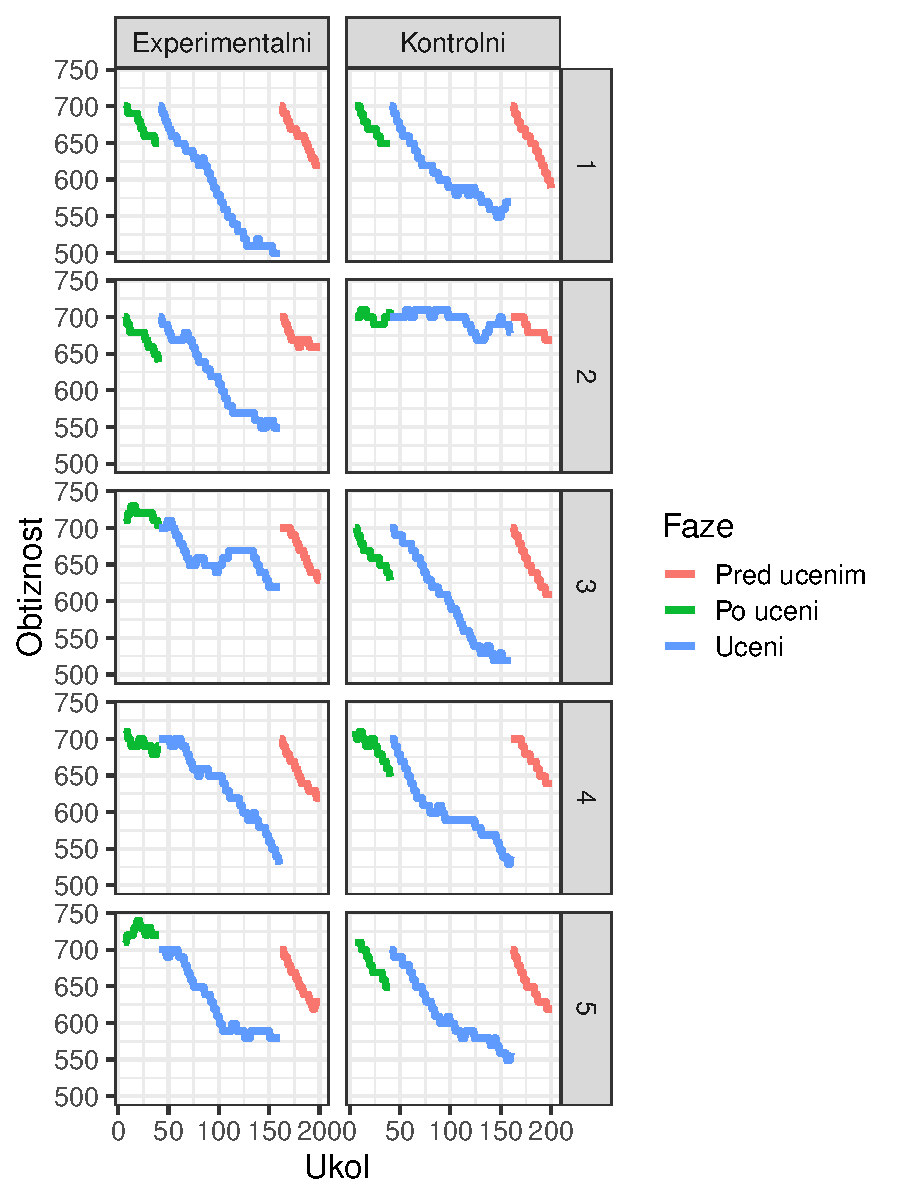
\includegraphics{graphs/difficulty_grid_all}}
\caption{Závislost obtížnosti na celkovém čísle úkolu.}
\end{figure}  
\end{center}
